\section{Prediction and Matching }
In this section, we will present the new method. At the first section, a new power budgeting method using model predictive method \cite{Wang:MPC_BOOK'09} will be introduced. At the second section, we will show the power matching method using task migration and DVFS \cite{MaWang:APCCAS'14}(dynamic voltage and frequency scaling). 
\subsection{New Power Budgeting Method for Dark Silicon}
In Dark Silion problems, not all the cores are active, because of the high power density of static power. So the cores are divided into two parts: active and inactive cores. And we want the temperature of the active cores close to the safe temperature (target temperature). Because at the target temperature, the performance of the active cores are the highest. If the cores' temperture go beyond the target temperature, dynamic thermal management will be triggered. And then the performance of the cores will be lowered. However, the ordinary dynamic thermal management will lead to overheated cores and/or overcooled cores because of lack of theoretical support. The new power budgeting method is to find the best distribution of the active cores that leads to the maximum power with the temperature of the cores all below the target temperature.

 
And in this work, we use model prediction method to predict the power of the cores and to guide us to budget the power.
   The basic idea of the new power budgeting method is to predict the appropriate power to make the active cores near or close to the target temperature. As there are active cores and inactive cores, we need to divide the temperature into two parts and we only care about the temperature of the active cores.  
  And we assume that after a few time steps the temperature of the active cores are close to or just the target temperature, and are written in a vector as 
\begin{equation}
\label{G}
\begin{split}
T=[t^T,t^T,\dotsb,t^T]^T \in R^{mN_p \times 1},\\
\end{split}
\end{equation}
In this vector, $T \in R^{m\times 1} $ means the target temperature of each core, $N_p$ stands for a time frame from current to the $N_p$ steps into the future, and is called the prediction horizon. What's important is that, $T$ contains the expected temperature not only the active cores but also the inactive cores. 
And the predicted temperature of the cores at future time steps can be written as
\begin{equation}
\label{y}
\begin{split}
T_c=[t_c(k+1|k)^T,t_c(k+2|k)^T,\dotsb,t_c(k+N_p|k)^T]^T, \\
\end{split}
\end{equation}
where $t_c(k+j|k)$ is the predicted core temperatures at time $k+j$ using the power of current time $k$.
$T_r$ also contains all the cores' temperature.
 And we use 
\begin{equation}
\label{Y}
\begin{split}
T_c(k)=Mt_a(k)+ N( p(k)-p(k-1)),\\
\end{split}
\end{equation}
 to compute the predicted temperature using power information at current time step.
where the variables are: 
\begin{equation}
\label{V}
\begin{split}
&M=\begin{bmatrix} CA \\ CA^2\\ \dotsc\\ CA^{N_p} \end{bmatrix}, N=\begin{bmatrix} CB \\CAB \\CA^2B \\ \dotsc \\ CA^{N_p-1}B \end{bmatrix},\\
&A=\begin{bmatrix} A_m & 0_m\\C_cA_m & I \end{bmatrix},B=\begin{bmatrix} B_m\\C_cB_m \end{bmatrix},\\
&C=\begin{bmatrix} 0_m & I \end{bmatrix},t_r(k)=\begin{bmatrix} t_c(k)-t_c(k-1) \\t_c(k) \end{bmatrix}.
\end{split}
\end{equation}

 To minimize the difference, we use the optimization \cite{Wang:MPC_BOOK'09}


\begin{equation}
\begin{split}
\text{minimize} &~~~~\parallel T-T_c \parallel_2\\
\text{subject to} &~~~~ card(p(k))=j,T>=Y,
\end{split}
\end{equation}
where $T_c$ is a function of $p(k)$. 
The first constraint is to guarantee the number of acitve cores and the second constraint is to make sure that each cores temperature will not go beyond the target temperature. $card$ is the cardinality function and its output is the number of nonzero components.
However, we only want the temperature of the active cores to reach the target temperature. And the only variable of the optimization is the power at current time step $k$. And the optimization \cite{Stephen:Convex_BOOK'09} is changed to
%\begin{equation}
%\begin{split}

%\end{split}
%\end{equation}


\begin{equation}
\begin{split}
\label{op_c} 
\text{minimize} &~~~\parallel Np(k)-e \parallel_2\\
\text{subject to} &~~~~card(p(k))=j,Np(k)-e<=0,
\end{split}
\end{equation}
where $e=T-Mt_{a}(k)+Np(k-1)$
,  $j$ means the number of active cores. So this optimization is turned to be an regressor selection problem. But to solve this regressor selection problem is too time consuming. So we use the equal formulation 

\begin{equation}
\begin{split}
\label{op_f} 
\text{minimize}  &~~~\parallel Np(k)-e \parallel_2\\
\text{subject to}  &~~~\parallel p(k) \parallel _1 < \alpha,Np(k)-e<=0,
\end{split}
\end{equation}
where
$\alpha$ is a positive number, and we change the value of $\alpha$ to fit the constraint $card(p(k))=j$. And we can using convex optimization methods \cite{Stephen:Convex_BOOK'09} to solve the power $p(k)$.


\subsection{Optimal Thermal Management Scheme}
After we get the predicted power $p(k)$ at time step $k$ , we always want the real power $\hat{p}(k)$ at time step $k$ to be the same with $p(k)$ which will make the best result. However, it is impossible in real conditions, what we can expect is that our $\hat{p}(k)$ mostly close to $p(k)$ and the temperature of all the cores is inside the target temperature. Based on this purpose, task migration and DVFS are employed in our matching method.


 Our matching method is based on the Hungarian algorithm \cite{Kuhn:NRLQ'55}. Hungarian method is a combinatorial optimization algorithm that solves the assignment problem in polynomial time, witch is suitable for our matching problem.

\subsubsection{Matching method with task migration}

Our matching method is to use Hungrian algorithm to find the smallest difference between the predicted power $p_a(k)$ and $\hat{p}_{b}(k)$. 
At first, we build a weighted complete bipartite graph at time step $k$, $G=(p(k),\hat{p}(k),E)$, where the vertex sets are $p(k)=\{p_1(k),p_2(k), \dotsc ,p_n(k)\}$,$\hat{p}(k)=\{\hat{p}_{1}(k),\hat{p}_{2}(k), \dotsc ,\hat{p}_{n}(k)\}$, and the edge set $E \in R^{n\times n}$ is a square matrix whose entries $e_{ab}$ are the difference of the predicted power at core $a$ and the former power at core $b$, $a,b$ are integers which means the position of the cores, like $e_{11}$ in fig. \ref{wei} shows.


\begin{figure}
  \centering
     {
       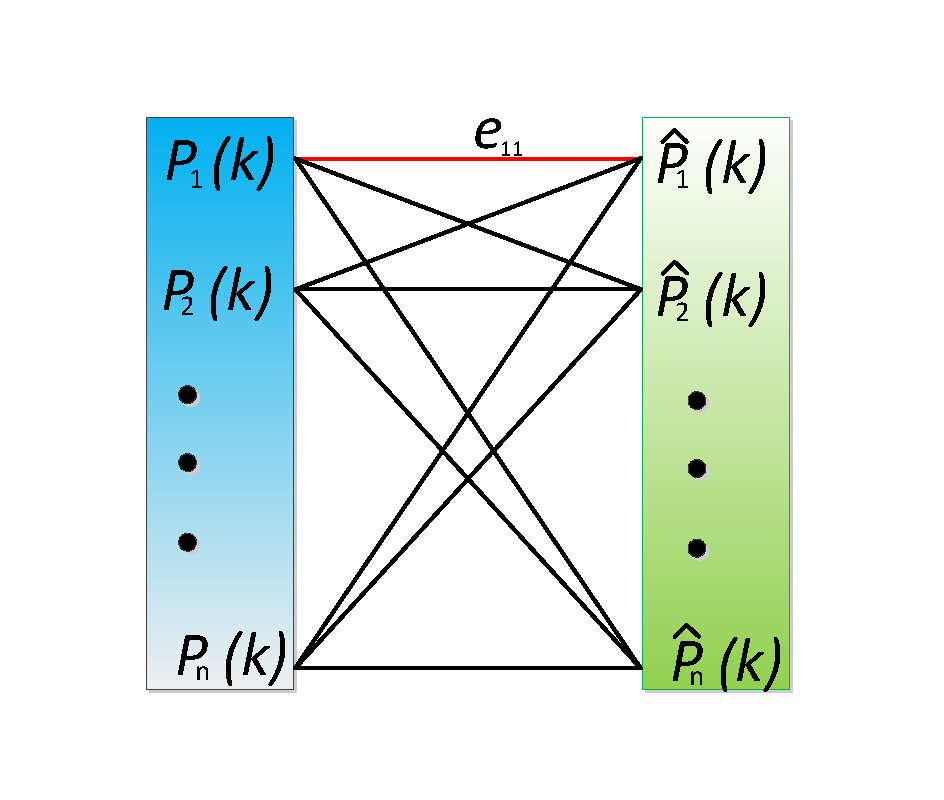
\includegraphics[width=0.4\textwidth]{fig/wei}
     }
     \caption{Example of task migration}\label{wei}
\end{figure}


 A threshold is set and any weight $e_{ab}$ smaller than the threshold shows the possibility of the exchange the power $p_a(k)$ and $\hat{p}_{b}(k)$.


\begin{equation}
\label{w}
e_{ab}=\left\{
\begin{aligned}
&  p_a(k)-\hat{p}_{b}(k)  &\quad p_a(k) >= \hat{p}_{b}(k),\\
& inf  &p_a(k) < \hat{p}_{b}(k).
\end{aligned}
\right.
\end{equation}


If $\hat{p}_{b}(k)$ is bigger than $p_a(k)$, which means the real power we add to core $a$ is greater than its predicted power, then we take the risk that the temperature of one or more core will go beyond the target which may trigger the inside dynamic thermal management, which may lower the performance.
As the exchange of the lower predicted power $p_c(k)$ and the higher former power$\hat{p}_{d}(k)$ is unacceptable where $c$ and $d$ is the position index, we assign the corresponding weight $e_{cd}$ to be infinite, which is far beyond the threshold.


The computation complexity of the Hungrian algorithm is $\mathcal{O} (n^{3})$ at least. However, in dark silicon problems the number of active cores $j$ is much smaller than the number of all the cores $n$. So we just consider the match between $j$ cores and the computation time decreases greatly. 







\begin{figure}
  \centering
     {
       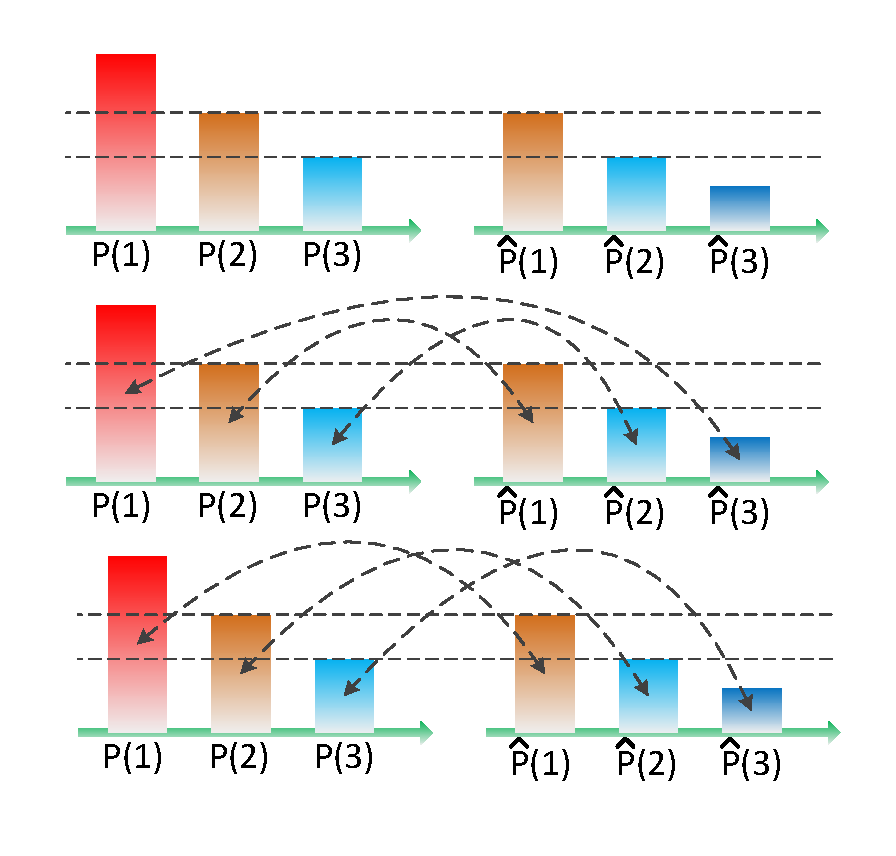
\includegraphics[width=0.4\textwidth]{fig/moderate}
     }
     \caption{Example of task migration}\label{moderate}
\end{figure}
 And there is one case like Fig.\ref{moderate} shows, $p(1)-p(3)$ means the predicted power, and $\hat{p}(1)-\hat{p}(3)$ means the current power waiting to be matched. We use double-headed arrow to stand for the matching. There exists two possible matchings based on our temperature constraint: the first is$[p(2) \hat{p}(1)]$, $[p(3) \hat{p}(2)]$, $[p(1) \hat{p}(3)]$ , the second is $[p(1) \hat{p}(1)]$ , $[p(2) \hat{p}(2)]$ , $[p(3) \hat{p}(3)]$. The first matching is generated with the hungarian method, which will cause one very low temperature on $\hat{p}(3)$. And the second matching is the moderate matching, which will cause moderate temperature of the three cores. In our view, the second matching is better. And if there exists the possiblity of the two matchings we choose the second one.
 
\subsubsection{Matching method with DVFS}

Only using task migration may guarantee the performance at some situations. However, if there are heavy load tasks, these power consuming task will cause high temperatures beyond the target temperature, which we cannot find corresponding cores to match them. We call these powers as ``left'' cores. For these powers, there are not positions that are fit for them. Because in any position these core's temperatures will go beyond the target temperature.


For these powers and tasks, DVFS is a must to handle the problem.
At first, we collect the left powers $\overline{p_a(k)}$ and $\overline{\hat{p}_{b}(k)}$. There are two cases that will make task migration unuseful. And we also find ways to handle them.


Case one:
 in this case, the number of heavy load tasks are far more than the number of light load tasks. At first, we calculate the average of  $\overline{p_a(k)}$ and $\overline{\hat{p}_{b}(k)}$. The average value of $\overline{p_a(k)}$ and $\overline{\hat{p}_b(k)}$ is $avg(\overline{p_a(k)})$ and $avg(\overline{\hat{p}_b(k)})$.  In case one $avg(\overline{p_a(k)})<avg(\overline{\hat{p}_{b}(k)})$, and we use the ratio
\begin{equation}\label{r_dvfs}
\gamma=\frac{avg(\overline{p_a(k)})}{ avg(\overline{\hat{p}_{b}(k)})}, 
\end{equation}
to scale the power, base on the realtionship
\begin{equation}\label{r_dvfs}
p\sim f^3,
\end{equation}
where $p$ means the power and $f$ means the frequency.


Case two:
in this case, the number of heavy load cores is nearly the same with the number of light load cores. In order to handle this, we set the threshold to be infinite to make all the leftovers matched. For a matched pair $[\overline{p_a(k)} \overline{\hat{p}_{b}(k)}]$, if $\overline{p_a(k)}>\overline{\hat{p}_{b}(k)}$. We just the exchange the power. Because it will not go beyond the target temperature. On the other hand, we can use the ratio
\begin{equation}\label{r_dvfs}
\gamma=\frac{\overline{p_a(k)}}{\overline{\hat{p}_{b}(k)}}, 
\end{equation}
to scale the power of $\overline{\hat{p}_{b}(k)}$ and exchange the pair.


And we use task migration and the two cases' DVFS iteratively to get the best distribution of the power.
